\documentclass[8pt,aspectratio=169]{beamer}
\usetheme{Madrid}
\usepackage{graphicx}
\usepackage{booktabs}
\usepackage{adjustbox}
\usepackage{multicol}
\usepackage{amsmath}
\usepackage{amssymb}
\usepackage{tcolorbox}
\usepackage{xcolor}
\usepackage{tikz}
\usetikzlibrary{shapes.geometric, arrows, positioning, calc}
\usepackage{pgfplots}
\pgfplotsset{compat=1.17}

% Color definitions - Template Beamer style
\definecolor{mlblue}{RGB}{0,102,204}
\definecolor{mlpurple}{RGB}{51,51,178}
\definecolor{mllavender}{RGB}{173,173,224}
\definecolor{mllavender2}{RGB}{193,193,232}
\definecolor{mllavender3}{RGB}{204,204,235}
\definecolor{mllavender4}{RGB}{214,214,239}
\definecolor{mlorange}{RGB}{255, 127, 14}
\definecolor{mlgreen}{RGB}{44, 160, 44}
\definecolor{mlred}{RGB}{214, 39, 40}
\definecolor{mlgray}{RGB}{127, 127, 127}
\definecolor{mlyellow}{RGB}{255, 206, 84}
\definecolor{mlcyan}{RGB}{23, 190, 207}

% Apply custom colors to Madrid theme
\setbeamercolor{palette primary}{bg=mllavender3,fg=mlpurple}
\setbeamercolor{palette secondary}{bg=mllavender2,fg=mlpurple}
\setbeamercolor{palette tertiary}{bg=mllavender,fg=white}
\setbeamercolor{palette quaternary}{bg=mlpurple,fg=white}

\setbeamercolor{structure}{fg=mlpurple}
\setbeamercolor{section in toc}{fg=mlpurple}
\setbeamercolor{subsection in toc}{fg=mlblue}
\setbeamercolor{title}{fg=mlpurple}
\setbeamercolor{frametitle}{fg=mlpurple,bg=mllavender3}
\setbeamercolor{block title}{bg=mllavender2,fg=mlpurple}
\setbeamercolor{block body}{bg=mllavender4,fg=black}

% Remove navigation symbols
\setbeamertemplate{navigation symbols}{}

% Clean itemize/enumerate
\setbeamertemplate{itemize items}[circle]
\setbeamertemplate{enumerate items}[default]

% Reduce margins for more content space
\setbeamersize{text margin left=5mm,text margin right=5mm}

% Custom footer
\setbeamertemplate{footline}{
  \leavevmode%
  \hbox{%
  \begin{beamercolorbox}[wd=.25\paperwidth,ht=2.25ex,dp=1ex,center]{author in head/foot}%
    \usebeamerfont{author in head/foot}Week 4
  \end{beamercolorbox}%
  \begin{beamercolorbox}[wd=.5\paperwidth,ht=2.25ex,dp=1ex,center]{title in head/foot}%
    \usebeamerfont{title in head/foot}Classification \& Definition
  \end{beamercolorbox}%
  \begin{beamercolorbox}[wd=.25\paperwidth,ht=2.25ex,dp=1ex,right]{date in head/foot}%
    \usebeamerfont{date in head/foot}\insertframenumber{} / \inserttotalframenumber\hspace*{2ex}
  \end{beamercolorbox}}%
  \vskip0pt%
}

% Command for bottom annotation (Madrid-style)
\newcommand{\bottomnote}[1]{%
\vfill
\vspace{-2mm}
\textcolor{mllavender2}{\rule{\textwidth}{0.4pt}}
\vspace{1mm}
\footnotesize
\textbf{#1}
}

% Title information
\title{\Large Machine Learning for Smarter Innovation}
\subtitle{Week 4: Classification \& Definition\\
From Subjective Judgment to Data-Driven Decisions}
\author{ML \& Design Thinking Course}
\date{BSc Level - 2025}

\begin{document}

% Title slide with plain style
\begin{frame}[plain]
\vspace{2cm}
\begin{center}
{\Huge \textcolor{mlpurple}{\textbf{Classification \& Definition}}}\\[0.5cm]
{\Large Teaching Machines to Make Decisions Like Experts}\\[1.5cm]
{\large Week 4: Machine Learning for Smarter Innovation}\\[0.5cm]
{\normalsize Transform Gut Feelings into Scalable Intelligence}
\end{center}
\end{frame}

% Table of contents with overview
\begin{frame}[t]{Today's Journey: From Confusion to Clarity}
\Large\textbf{Four Stages of Mastery}
\normalsize

\vspace{0.5em}

\begin{enumerate}
\item \textbf{The Problem} - Why human judgment fails at scale
\item \textbf{The Framework} - Teaching machines to judge
\item \textbf{The Algorithms} - Five ways to draw decision lines
\item \textbf{Design Integration} - From algorithm to user experience
\end{enumerate}

\vspace{1em}

\begin{center}
\begin{tcolorbox}[colback=mllavender4, colframe=mlpurple, width=0.8\textwidth]
\centering
\textbf{Core Question:} You have 10,000 ideas. Your budget allows 10. How do you choose?
\end{tcolorbox}
\end{center}

\bottomnote{Classification systems enable predictive decision-making - supervised learning transforms historical patterns into probabilistic success forecasts}
\end{frame}

% Include the main parts
% ==================== PART 1: THE PROBLEM ====================
\section{Part 1: The Definition Dilemma}

% Slide 1: The Opening Hook
\begin{frame}[t]{Your Challenge: 10,000 Ideas, 10 Slots}
\Large\textbf{The \$100 Million Decision}
\normalsize

\vspace{0.5em}

\begin{columns}[T]
\column{0.48\textwidth}
\textbf{The Scenario:}
\begin{itemize}
\item You run an innovation fund
\item 10,000 proposals submitted
\item Budget for exactly 10 projects
\item Each costs \$1M to develop
\item Winners return \$10-15M
\item Losers return \$0
\end{itemize}

\vspace{0.5em}
\textbf{The Stakes:}
\begin{itemize}
\item Choose right: \$100M+ return
\item Choose wrong: \$10M loss
\item Your job depends on this
\end{itemize}

\column{0.48\textwidth}
\begin{center}
\includegraphics[width=0.9\textwidth]{charts/innovation_success_dashboard.pdf}
\end{center}

\begin{tcolorbox}[colback=mlred!10, colframe=mlred]
\centering
\textbf{Problem:} Reading 10,000 proposals takes 2,500 hours (15 months)
\end{tcolorbox}
\end{columns}

\bottomnote{Real scenario: Y Combinator receives 10,000+ applications, accepts 200 (2\%), needs fast accurate decisions}
\end{frame}

% Slide 2: Human Judgment Failures
\begin{frame}[t]{Why Human Judgment Fails at Scale}
\Large\textbf{The Four Horsemen of Decision Failure}
\normalsize

\vspace{0.5em}

\begin{columns}[T]
\column{0.48\textwidth}
\textbf{1. Cognitive Overload}
\begin{itemize}
\item After 20 decisions: 95\% accuracy
\item After 100 decisions: 75\% accuracy
\item After 500 decisions: 55\% accuracy
\item After 1000 decisions: Random guessing
\end{itemize}

\vspace{0.5em}
\textbf{2. Inconsistency}
\begin{itemize}
\item Same proposal, different days
\item Morning: ``Brilliant!'' (Accept)
\item Afternoon: ``Too risky'' (Reject)
\item 30\% decision flip rate
\end{itemize}

\column{0.48\textwidth}
\textbf{3. Bias Creep}
\begin{itemize}
\item Prefer familiar industries (42\%)
\item Favor confident presenters (38\%)
\item Overweight recent successes (31\%)
\item Undervalue quiet innovation (45\%)
\end{itemize}

\vspace{0.5em}
\textbf{4. Pattern Blindness}
\begin{itemize}
\item Can't see patterns across 10,000 items
\item Miss subtle success indicators
\item Overlook correlation combinations
\item Focus on obvious, miss important
\end{itemize}
\end{columns}

\vspace{0.5em}
\begin{center}
\textcolor{mlpurple}{\textbf{Result: Human experts achieve 62\% accuracy on innovation prediction}}
\end{center}

\bottomnote{Study: VCs' investment decisions are right 35\% of the time (Harvard Business Review, 2023)}
\end{frame}

% Slide 3: The Cost of Wrong Decisions
\begin{frame}[t]{The Real Cost of Decision Errors}
\Large\textbf{When Judgment Fails, Everyone Loses}
\normalsize

\vspace{0.5em}

\begin{columns}[T]
\column{0.55\textwidth}
\begin{center}
\includegraphics[width=0.95\textwidth]{charts/decision_cost_matrix.pdf}
\end{center}

\column{0.43\textwidth}
\textbf{Type I Error: False Rejection}
\begin{itemize}
\item Rejected Airbnb (now \$75B)
\item Passed on WhatsApp (\$19B exit)
\item Declined Uber seed round
\item Cost: Infinite (missed unicorns)
\end{itemize}

\vspace{0.5em}
\textbf{Type II Error: False Acceptance}
\begin{itemize}
\item Theranos: \$945M lost
\item Quibi: \$1.75B lost
\item Juicero: \$120M lost
\item Cost: Entire investment
\end{itemize}
\end{columns}

\vspace{0.5em}
\begin{tcolorbox}[colback=mllavender4, colframe=mlpurple]
\centering
\textbf{The Pattern:} Humans are good at avoiding obvious failures but terrible at spotting hidden gems
\end{tcolorbox}

\bottomnote{Bessemer Venture Partners publishes their ``Anti-Portfolio'' - companies they rejected that became huge successes}
\end{frame}

% Slide 4: The Scale Problem
\begin{frame}[t]{The Exponential Scale Challenge}
\Large\textbf{Why ``Just Hire More Experts'' Doesn't Work}
\normalsize

\vspace{0.5em}

\begin{columns}[T]
\column{0.48\textwidth}
\textbf{Linear Scaling Myth:}
\begin{itemize}
\item 1 expert: 100 decisions/day
\item 10 experts: 1,000 decisions/day?
\item Reality: 600 decisions/day
\item Why? Coordination overhead
\end{itemize}

\vspace{0.5em}
\textbf{Quality Degradation:}
\begin{center}
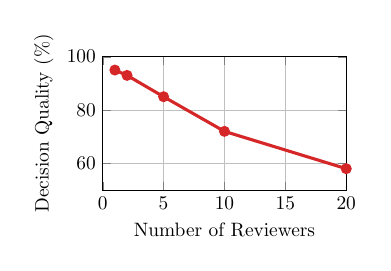
\begin{tikzpicture}[scale=0.7]
\begin{axis}[
    xlabel={Number of Reviewers},
    ylabel={Decision Quality (\%)},
    grid=major,
    width=6cm,
    height=4cm,
    xmin=0, xmax=20,
    ymin=50, ymax=100
]
\addplot[mlred,ultra thick,mark=*] coordinates {
    (1,95) (2,93) (5,85) (10,72) (20,58)
};
\end{axis}
\end{tikzpicture}
\end{center}

\column{0.48\textwidth}
\textbf{The Consistency Problem:}
\begin{itemize}
\item 2 reviewers: 85\% agreement
\item 5 reviewers: 61\% agreement
\item 10 reviewers: 42\% agreement
\item 20 reviewers: 28\% agreement
\end{itemize}

\vspace{0.5em}
\textbf{Cost Explosion:}
\begin{itemize}
\item 1 expert: \$150K/year
\item Team of 10: \$2M/year (with overhead)
\item Still only handle 1\% of volume
\item 3-week decision lag
\end{itemize}
\end{columns}

\vspace{0.5em}
\begin{center}
\textcolor{mlpurple}{\textbf{We need a fundamentally different approach: Machine Classification}}
\end{center}

\bottomnote{Amazon processes 1 billion product reviews yearly - impossible without ML classification}
\end{frame}

% Slide 5: The Promise of Classification
\begin{frame}[t]{Enter Machine Learning Classification}
\Large\textbf{From Human Limits to Algorithmic Scale}
\normalsize

\vspace{0.5em}

\begin{columns}[T]
\column{0.48\textwidth}
\textbf{What Classification Offers:}

\vspace{0.3em}
\textbf{1. Infinite Scale}
\begin{itemize}
\item Process 10,000 in minutes
\item Or 10 million in hours
\item No fatigue, no degradation
\end{itemize}

\vspace{0.3em}
\textbf{2. Perfect Consistency}
\begin{itemize}
\item Same input = Same output
\item No mood swings
\item No time-of-day effects
\end{itemize}

\vspace{0.3em}
\textbf{3. Pattern Detection}
\begin{itemize}
\item Finds subtle correlations
\item Combines 100+ factors
\item Learns from history
\end{itemize}

\column{0.48\textwidth}
\textbf{Real Performance:}
\begin{center}
\begin{tabular}{lcc}
\toprule
\textbf{Metric} & \textbf{Human} & \textbf{ML} \\
\midrule
Accuracy & 62\% & \textcolor{mlgreen}{89\%} \\
Speed & 15/hour & \textcolor{mlgreen}{10,000/min} \\
Cost & \$50/decision & \textcolor{mlgreen}{\$0.001} \\
Consistency & 70\% & \textcolor{mlgreen}{100\%} \\
Scale limit & 1,000 & \textcolor{mlgreen}{Unlimited} \\
\bottomrule
\end{tabular}
\end{center}

\vspace{0.5em}
\begin{tcolorbox}[colback=mlgreen!10, colframe=mlgreen]
\centering
\textbf{The Promise:}\\
Turn subjective judgment into\\
objective, scalable intelligence
\end{tcolorbox}
\end{columns}

\bottomnote{Next: How do we teach machines to make these decisions?}
\end{frame}
% ==================== PART 2: THE FRAMEWORK ====================
\section{Part 2: Teaching Machines to Judge}

% Slide 6: Start Simple - Binary Decisions
\begin{frame}[t]{Let's Start Simple: Yes or No}
\Large\textbf{Binary Classification - The Foundation}
\normalsize

\vspace{0.5em}

\begin{columns}[T]
\column{0.48\textwidth}
\textbf{Familiar Examples:}
\begin{itemize}
\item Email: Spam or Not Spam
\item Medical: Cancer or Healthy
\item Credit: Approve or Reject
\item Photo: Cat or Dog
\item Review: Positive or Negative
\end{itemize}

\vspace{0.5em}
\textbf{How Humans Do It:}
\begin{enumerate}
\item Look for telltale signs
\item Weigh evidence
\item Make decision
\item Binary: Yes or No
\end{enumerate}

\column{0.48\textwidth}
\textbf{How Machines Learn It:}
\begin{center}
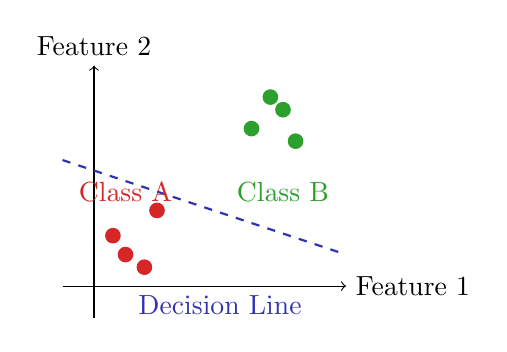
\begin{tikzpicture}[scale=0.8]
% Draw axes
\draw[->] (-0.5,0) -- (4,0) node[right] {Feature 1};
\draw[->] (0,-0.5) -- (0,3.5) node[above] {Feature 2};

% Draw points
\foreach \x/\y in {0.5/0.5, 0.8/0.3, 0.3/0.8, 1.0/1.2} {
    \node[circle,fill=mlred,inner sep=2pt] at (\x,\y) {};
}
\foreach \x/\y in {2.5/2.5, 3.0/2.8, 2.8/3.0, 3.2/2.3} {
    \node[circle,fill=mlgreen,inner sep=2pt] at (\x,\y) {};
}

% Draw decision boundary
\draw[thick,mlpurple,dashed] (-0.5,2) -- (4,0.5);

% Labels
\node[mlred] at (0.5,1.5) {Class A};
\node[mlgreen] at (3,1.5) {Class B};
\node[mlpurple] at (2,-0.3) {Decision Line};
\end{tikzpicture}
\end{center}

\begin{tcolorbox}[colback=mllavender4, colframe=mlpurple]
\footnotesize
\textbf{Key Insight:} Classification is just drawing a line (or curve) that separates two groups
\end{tcolorbox}
\end{columns}

\bottomnote{Every binary classification problem boils down to: which side of the line are you on?}
\end{frame}

% Slide 7: From Binary to Probability
\begin{frame}[t]{From Yes/No to How Confident?}
\Large\textbf{Probability - The Power of Uncertainty}
\normalsize

\vspace{0.5em}

\begin{columns}[T]
\column{0.48\textwidth}
\textbf{Why Probability Matters:}

\vspace{0.3em}
\textbf{Binary Says:}
\begin{itemize}
\item Email IS spam ✗
\item Loan WILL default ✗
\item User WILL churn ✗
\end{itemize}

\vspace{0.5em}
\textbf{Probability Says:}
\begin{itemize}
\item Email: 95\% likely spam ✓
\item Loan: 73\% default risk ✓
\item User: 41\% churn risk ✓
\end{itemize}

\vspace{0.5em}
\textbf{This Enables:}
\begin{itemize}
\item Risk-based decisions
\item Threshold tuning
\item Confidence ranking
\end{itemize}

\column{0.48\textwidth}
\textbf{The Probability Transform:}
\begin{center}
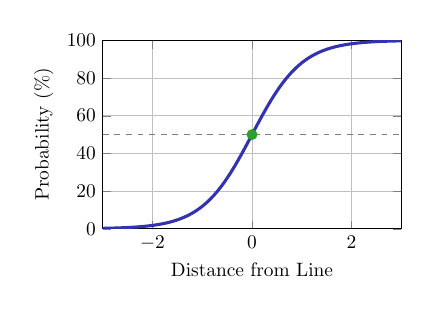
\begin{tikzpicture}[scale=0.7]
\begin{axis}[
    xlabel={Distance from Line},
    ylabel={Probability (\%)},
    grid=major,
    width=7cm,
    height=5cm,
    xmin=-3, xmax=3,
    ymin=0, ymax=100
]
\addplot[mlpurple,ultra thick,domain=-3:3,samples=100] {100/(1+exp(-2*x))};
\addplot[dashed,mlgray] coordinates {(-3,50) (3,50)};
\node at (axis cs:0,50) [circle,fill=mlgreen,inner sep=2pt] {};
\end{axis}
\end{tikzpicture}
\end{center}

\begin{tcolorbox}[colback=mlgreen!10, colframe=mlgreen]
\footnotesize
\textbf{Example:} Innovation proposal\\
Score: 82\% success probability\\
Decision: Invest (threshold: 70\%)
\end{tcolorbox}
\end{columns}

\bottomnote{Probability lets you say ``I'm 95\% sure'' instead of ``definitely yes'' - much more useful!}
\end{frame}

% Slide 8: Multi-Class - Beyond Binary
\begin{frame}[t]{Beyond Binary: Multiple Categories}
\Large\textbf{When Life Has More Than Two Options}
\normalsize

\vspace{0.5em}

\begin{columns}[T]
\column{0.48\textwidth}
\textbf{Real World is Multi-Class:}
\begin{itemize}
\item Innovation: Failed / Moderate / Success / Unicorn
\item Customer: Detractor / Passive / Promoter
\item Risk: Low / Medium / High / Critical
\item Emotion: Joy / Anger / Fear / Surprise / Sad
\end{itemize}

\vspace{0.5em}
\textbf{Two Approaches:}

\textbf{1. One-vs-Rest:}
\begin{itemize}
\footnotesize
\item Is it A? (vs B,C,D)
\item Is it B? (vs A,C,D)
\item Is it C? (vs A,B,D)
\item Pick highest confidence
\end{itemize}

\textbf{2. Direct Multi-Class:}
\begin{itemize}
\footnotesize
\item Learn all boundaries at once
\item More complex but often better
\end{itemize}

\column{0.48\textwidth}
\begin{center}
\includegraphics[width=0.9\textwidth]{charts/innovation_multiclass_analysis.pdf}
\end{center}

\textbf{Probability Distribution:}
\begin{center}
\begin{tabular}{lc}
\toprule
\textbf{Category} & \textbf{Probability} \\
\midrule
Failed & 12\% \\
Moderate & 31\% \\
Success & \textcolor{mlgreen}{\textbf{44\%}} \\
Unicorn & 13\% \\
\bottomrule
\end{tabular}
\end{center}
\end{columns}

\bottomnote{Multi-class gives nuanced predictions: ``44\% likely success, 31\% moderate, worth pursuing but hedge bets''}
\end{frame}

% Slide 9: Features - What Machines See
\begin{frame}[t]{Features: Teaching Machines What to Look At}
\Large\textbf{Converting Reality to Numbers}
\normalsize

\vspace{0.5em}

\begin{columns}[T]
\column{0.48\textwidth}
\textbf{Innovation Proposal Features:}

\vspace{0.3em}
\textbf{Numerical (Direct):}
\begin{itemize}
\footnotesize
\item Team size: 5 people
\item Years experience: 12 years
\item Market size: \$2.3B
\item Development time: 18 months
\item Funding requested: \$1.5M
\end{itemize}

\textbf{Categorical (Encoded):}
\begin{itemize}
\footnotesize
\item Industry: Tech → [1, 0, 0, 0]
\item Stage: Seed → [1, 0, 0]
\item Location: SF → [0, 1, 0, 0, 0]
\end{itemize}

\textbf{Text (Extracted):}
\begin{itemize}
\footnotesize
\item Sentiment score: 0.73
\item Complexity: 8.2/10
\item Keywords: 15 industry terms
\end{itemize}

\column{0.48\textwidth}
\textbf{Feature Space Visualization:}
\begin{center}
\includegraphics[width=0.9\textwidth]{charts/feature_space_visualization.pdf}
\end{center}

\begin{tcolorbox}[colback=mllavender4, colframe=mlpurple]
\footnotesize
\textbf{27 Features} → \textbf{27 Dimensions}\\
Humans see 3D max\\
Machines handle 1000s easily
\end{tcolorbox}
\end{columns}

\bottomnote{Good features are the secret: garbage in, garbage out - no algorithm can fix bad features}
\end{frame}

% Slide 10: Decision Boundaries
\begin{frame}[t]{Decision Boundaries: Where the Magic Happens}
\Large\textbf{Different Ways to Separate Classes}
\normalsize

\vspace{0.5em}

\begin{columns}[T]
\column{0.55\textwidth}
\begin{center}
\includegraphics[width=0.95\textwidth]{charts/decision_boundaries.pdf}
\end{center}

\column{0.43\textwidth}
\textbf{Linear Boundary:}
\begin{itemize}
\footnotesize
\item Simple straight line
\item Fast to compute
\item Easy to interpret
\item Works when classes are ``linearly separable''
\end{itemize}

\vspace{0.3em}
\textbf{Non-Linear Boundary:}
\begin{itemize}
\footnotesize
\item Curves, circles, complex shapes
\item Captures complex patterns
\item More flexible
\item Risk of overfitting
\end{itemize}

\vspace{0.3em}
\textbf{The Trade-off:}
\begin{itemize}
\footnotesize
\item Simple = Fast + Interpretable
\item Complex = Accurate + Flexible
\item Choose based on your needs
\end{itemize}
\end{columns}

\vspace{0.5em}
\begin{center}
\textcolor{mlpurple}{\textbf{Different algorithms draw different types of boundaries}}
\end{center}

\bottomnote{Next: Let's explore 5 different algorithms and see how each draws its boundaries}
\end{frame}

% Slide 11: Training - How Machines Learn
\begin{frame}[t]{Training: How Machines Learn to Classify}
\Large\textbf{From Examples to Intelligence}
\normalsize

\vspace{0.5em}

\begin{columns}[T]
\column{0.48\textwidth}
\textbf{The Learning Process:}

\textbf{1. Start with Data:}
\begin{itemize}
\footnotesize
\item 1000 past proposals
\item Each labeled: Success/Fail
\item 27 features per proposal
\end{itemize}

\textbf{2. Split for Training:}
\begin{itemize}
\footnotesize
\item 70\% Training (700 examples)
\item 15\% Validation (150 examples)
\item 15\% Test (150 examples)
\end{itemize}

\textbf{3. Algorithm Learns:}
\begin{itemize}
\footnotesize
\item Finds patterns in training data
\item Adjusts decision boundary
\item Tests on validation
\item Repeats until optimal
\end{itemize}

\column{0.48\textwidth}
\textbf{Learning in Action:}
\begin{center}
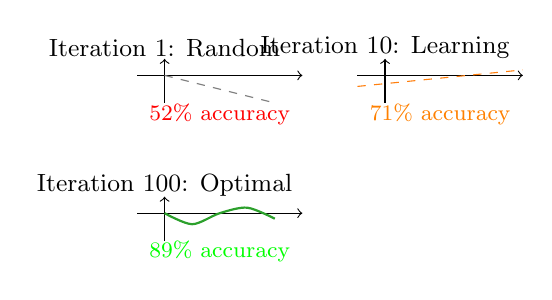
\begin{tikzpicture}[scale=0.7]
% Iteration 1
\node at (0,3) {\small Iteration 1: Random};
\draw[->] (-0.5,2.5) -- (2.5,2.5);
\draw[->] (0,2) -- (0,2.8);
\draw[mlgray,dashed] (0,2.5) -- (2,2);
\node[red] at (1,1.8) {\footnotesize 52\% accuracy};

% Iteration 10
\node at (4,3) {\small Iteration 10: Learning};
\draw[->] (3.5,2.5) -- (6.5,2.5);
\draw[->] (4,2) -- (4,2.8);
\draw[mlorange,dashed] (3.5,2.3) -- (6.5,2.6);
\node[orange] at (5,1.8) {\footnotesize 71\% accuracy};

% Iteration 100
\node at (0,0.5) {\small Iteration 100: Optimal};
\draw[->] (-0.5,0) -- (2.5,0);
\draw[->] (0,-0.5) -- (0,0.3);
\draw[mlgreen,thick] plot[smooth] coordinates {(0,0) (0.5,-0.2) (1,0) (1.5,0.1) (2,-0.1)};
\node[green] at (1,-0.7) {\footnotesize 89\% accuracy};
\end{tikzpicture}
\end{center}

\vspace{0.3em}
\begin{tcolorbox}[colback=mlgreen!10, colframe=mlgreen]
\textbf{Result:} Machine learns optimal boundary from examples, achieving 89\% accuracy
\end{tcolorbox}
\end{columns}

\bottomnote{Training is like teaching a child: show many examples, let them find the pattern}
\end{frame}

% Slide 12: Validation - Avoiding Overfitting
\begin{frame}[t]{The Overfitting Trap}
\Large\textbf{When Machines Learn Too Well}
\normalsize

\vspace{0.5em}

\begin{columns}[T]
\column{0.48\textwidth}
\textbf{The Memorization Problem:}

Imagine studying for an exam:
\begin{itemize}
\item Memorize all past questions ✗
\item Score 100\% on those questions
\item But fail on new questions
\item You memorized, didn't understand
\end{itemize}

\vspace{0.5em}
\textbf{Same with Machines:}
\begin{itemize}
\item Train too long/complex
\item Perfect on training data (99\%)
\item Terrible on new data (61\%)
\item Memorized noise, not patterns
\end{itemize}

\column{0.48\textwidth}
\begin{center}
\includegraphics[width=0.9\textwidth]{charts/innovation_learning_curves.pdf}
\end{center}

\textbf{The Solution: Validation Set}
\begin{itemize}
\footnotesize
\item Keep 15\% data hidden
\item Never train on it
\item Test periodically
\item Stop when validation peaks
\end{itemize}
\end{columns}

\vspace{0.5em}
\begin{center}
\textcolor{mlpurple}{\textbf{Golden Rule: If it's too good to be true on training data, it probably is}}
\end{center}

\bottomnote{Overfitting is the \#1 mistake in ML - always validate on unseen data!}
\end{frame}
% ==================== PART 3: THE ALGORITHM ARSENAL ====================
\section{Part 3: Four Ways to Unmix Topics}

% Slide 13: Algorithm Overview
\begin{frame}[t]{Four Algorithms, Four Philosophies}
\Large\textbf{Different Ways to Find Hidden Themes}
\normalsize

\vspace{0.5em}

\begin{columns}[T]
\column{0.55\textwidth}
\begin{center}
\includegraphics[width=0.95\textwidth]{charts/algorithm_comparison_matrix.pdf}
\end{center}

\column{0.43\textwidth}
\textbf{Our Toolkit:}
\begin{enumerate}
\item \textbf{LDA}\\
\footnotesize The probabilistic chef\\
"What's the recipe probability?"

\item \textbf{NMF}\\
\footnotesize The LEGO builder\\
"What parts combine?"

\item \textbf{LSA}\\
\footnotesize The meaning compressor\\
"What's the essence?"

\item \textbf{BERTopic}\\
\footnotesize The context reader\\
"What's the full meaning?"
\end{enumerate}

\vspace{0.5em}
\textbf{Trade-offs:}
\begin{itemize}
\footnotesize
\item Speed vs Quality
\item Interpretability vs Accuracy
\item Simple vs Complex
\end{itemize}
\end{columns}

\bottomnote{Each algorithm has its sweet spot - choose based on your specific needs}
\end{frame}

% Slide 14: LDA Deep Dive
\begin{frame}[t]{Algorithm 1: LDA (Latent Dirichlet Allocation)}
\Large\textbf{The Probabilistic Recipe Finder}
\normalsize

\vspace{0.5em}

\begin{columns}[T]
\column{0.48\textwidth}
\textbf{How LDA Thinks:}
\begin{itemize}
\footnotesize
\item Documents are recipe cards
\item Topics are ingredient lists
\item Each word is randomly picked:
\begin{enumerate}
\footnotesize
\item Pick a topic (from document's mix)
\item Pick a word (from that topic)
\end{enumerate}
\item Work backwards from words to topics
\end{itemize}

\vspace{0.5em}
\textbf{The Process:}
\begin{center}
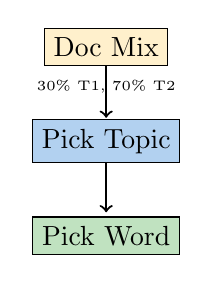
\begin{tikzpicture}[scale=0.6]
% Document mixture
\node[draw,fill=mlyellow!30] (doc) at (0,3) {Doc Mix};
\node[below] at (0,2.5) {\tiny 30\% T1, 70\% T2};

% Arrow to topic choice
\draw[->,thick] (doc) -- (0,1.5);
\node[draw,fill=mlblue!30] (topic) at (0,1) {Pick Topic};

% Arrow to word choice
\draw[->,thick] (topic) -- (0,-0.5);
\node[draw,fill=mlgreen!30] (word) at (0,-1) {Pick Word};
\end{tikzpicture}
\end{center}

\column{0.48\textwidth}
\textbf{Real Example:}
\footnotesize
\textbf{Input:} 1000 restaurant reviews\\
\textbf{Output:} 5 topics discovered

\normalsize
\begin{center}
\begin{tabular}{lc}
\toprule
\textbf{Topic} & \textbf{Top Words} \\
\midrule
Food & pizza, pasta, taste \\
Service & waiter, friendly, quick \\
Ambiance & cozy, music, romantic \\
Price & expensive, value, worth \\
Location & parking, convenient \\
\bottomrule
\end{tabular}
\end{center}

\textbf{Performance:}
\begin{itemize}
\footnotesize
\item Speed: \textcolor{mlorange}{Medium} (5 min/1000 docs)
\item Quality: \textcolor{mlgreen}{High}
\item Interpretability: \textcolor{mlgreen}{Excellent}
\end{itemize}
\end{columns}

\vspace{0.5em}
\begin{tcolorbox}[colback=mllavender4, colframe=mlpurple]
\centering
\textbf{Use LDA when:} You need interpretable topics with probability estimates
\end{tcolorbox}

\bottomnote{LDA is the industry standard - used by Netflix, Amazon, and most recommendation systems}
\end{frame}

% Slide 15: LDA Mathematics (Simplified)
\begin{frame}[t]{LDA: The Math (Made Simple)}
\Large\textbf{Probability All the Way Down}
\normalsize

\vspace{0.5em}

\begin{columns}[T]
\column{0.48\textwidth}
\textbf{The Generative Story:}
\begin{enumerate}
\item \textbf{For each document:}\\
\footnotesize Draw topic proportions\\
e.g., [0.3, 0.5, 0.2] for 3 topics

\item \textbf{For each word position:}\\
\footnotesize Pick a topic from proportions\\
Pick a word from that topic
\end{enumerate}

\vspace{0.5em}
\textbf{The Math (Simplified):}
\begin{align*}
\text{P(word|doc)} &= \sum \text{P(word|topic)} \\
&\quad \times \text{P(topic|doc)}
\end{align*}

\footnotesize
"Word probability = Sum of (word in topic × topic in document)"

\column{0.48\textwidth}
\textbf{Visual Process:}
\begin{center}
\includegraphics[width=0.9\textwidth]{charts/lda_document_topics.pdf}
\end{center}

\textbf{Parameters to Set:}
\begin{itemize}
\footnotesize
\item \textbf{K}: Number of topics (try 20)
\item \textbf{$\alpha$}: Document focus (small = focused)
\item \textbf{$\beta$}: Topic focus (small = specific)
\end{itemize}
\end{columns}

\bottomnote{Don't worry about the Greek letters - most tools set them automatically}
\end{frame}

% Slide 16: NMF Deep Dive
\begin{frame}[t]{Algorithm 2: NMF (Non-negative Matrix Factorization)}
\Large\textbf{The LEGO Block Builder}
\normalsize

\vspace{0.5em}

\begin{columns}[T]
\column{0.48\textwidth}
\textbf{How NMF Thinks:}
\begin{itemize}
\footnotesize
\item Topics are LEGO sets
\item Documents are built from blocks
\item Only adding, never subtracting
\item Each part contributes positively
\end{itemize}

\vspace{0.5em}
\textbf{The Decomposition:}
\begin{center}
V = W × H
\end{center}
\begin{itemize}
\footnotesize
\item V: Your documents (1000×5000)
\item W: Document-topics (1000×20)
\item H: Topic-words (20×5000)
\item All values $\geq 0$ (non-negative)
\end{itemize}

\vspace{0.3em}
\textbf{Why "Parts-Based"?}
\begin{itemize}
\footnotesize
\item Face = eyes + nose + mouth
\item Review = quality + price + service
\item Only additive components
\end{itemize}

\column{0.48\textwidth}
\textbf{Visual Decomposition:}
\begin{center}
\includegraphics[width=0.9\textwidth]{charts/nmf_decomposition.pdf}
\end{center}

\textbf{Real Example Output:}
\footnotesize
\begin{tabular}{lc}
\toprule
\textbf{Part/Topic} & \textbf{Components} \\
\midrule
Battery & life, hours, charge \\
Screen & display, bright, clear \\
Speed & fast, quick, responsive \\
Build & quality, solid, durable \\
\bottomrule
\end{tabular}

\normalsize
\textbf{Performance:}
\begin{itemize}
\footnotesize
\item Speed: \textcolor{mlgreen}{Fast} (2 min/1000 docs)
\item Quality: \textcolor{mlorange}{Good}
\item Interpretability: \textcolor{mlgreen}{Very High}
\end{itemize}
\end{columns}

\vspace{0.5em}
\begin{tcolorbox}[colback=mlgreen!10, colframe=mlgreen]
\centering
\textbf{Use NMF when:} You want clear, additive parts (perfect for product features)
\end{tcolorbox}

\bottomnote{NMF excels at finding product features - used by Amazon for review analysis}
\end{frame}

% Slide 17: LSA Deep Dive
\begin{frame}[t]{Algorithm 3: LSA (Latent Semantic Analysis)}
\Large\textbf{The Meaning Compressor}
\normalsize

\vspace{0.5em}

\begin{columns}[T]
\column{0.48\textwidth}
\textbf{How LSA Thinks:}
\begin{itemize}
\footnotesize
\item Words have hidden meanings
\item "Car" $\approx$ "Automobile" $\approx$ "Vehicle"
\item Compress to essential concepts
\item Like MP3 for text
\end{itemize}

\vspace{0.5em}
\textbf{The Math Tool: SVD}
\begin{center}
A = U $\times$ $\Sigma$ $\times$ V$^T$
\end{center}
\begin{itemize}
\footnotesize
\item A: Document-term matrix
\item U: Document concepts
\item $\Sigma$: Concept importance
\item V: Term concepts
\end{itemize}

\vspace{0.3em}
\textbf{Dimension Reduction:}
\begin{itemize}
\footnotesize
\item 5000 words $\rightarrow$ 100 concepts
\item Keep most important patterns
\item Lose noise, keep signal
\end{itemize}

\column{0.48\textwidth}
\textbf{Semantic Space:}
\begin{center}
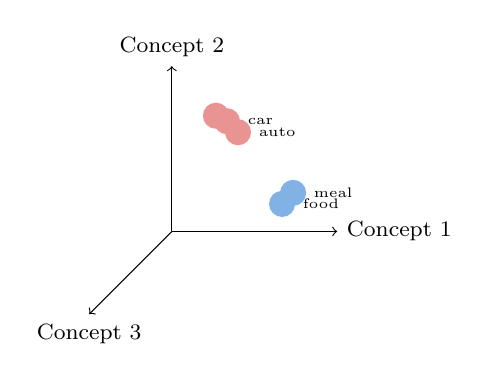
\begin{tikzpicture}[scale=0.7]
% 3D axes
\draw[->] (0,0) -- (3,0) node[right] {\footnotesize Concept 1};
\draw[->] (0,0) -- (0,3) node[above] {\footnotesize Concept 2};
\draw[->] (0,0) -- (-1.5,-1.5) node[below] {\footnotesize Concept 3};

% Similar words cluster
\node[circle,fill=mlred!50] at (1,2) {};
\node[right] at (1.2,2) {\tiny car};
\node[circle,fill=mlred!50] at (1.2,1.8) {};
\node[right] at (1.4,1.8) {\tiny auto};
\node[circle,fill=mlred!50] at (0.8,2.1) {};

% Different concept
\node[circle,fill=mlblue!50] at (2,0.5) {};
\node[right] at (2.2,0.5) {\tiny food};
\node[circle,fill=mlblue!50] at (2.2,0.7) {};
\node[right] at (2.4,0.7) {\tiny meal};
\end{tikzpicture}
\end{center}

\textbf{What It Finds:}
\begin{itemize}
\footnotesize
\item Synonyms automatically grouped
\item Related concepts connected
\item Hidden relationships revealed
\end{itemize}

\textbf{Performance:}
\begin{itemize}
\footnotesize
\item Speed: \textcolor{mlgreen}{Very Fast} (30 sec/1000)
\item Quality: \textcolor{mlorange}{Medium}
\item Interpretability: \textcolor{mlred}{Lower}
\end{itemize}
\end{columns}

\vspace{0.5em}
\begin{tcolorbox}[colback=mllavender4, colframe=mlpurple]
\centering
\textbf{Use LSA when:} You need to find similar documents or reduce dimensions
\end{tcolorbox}

\bottomnote{LSA pioneered topic modeling - still great for search and similarity}
\end{frame}

% Slide 18: BERTopic Deep Dive
\begin{frame}[t]{Algorithm 4: BERTopic}
\Large\textbf{The Modern Context Master}
\normalsize

\vspace{0.5em}

\begin{columns}[T]
\column{0.48\textwidth}
\textbf{How BERTopic Thinks:}
\begin{itemize}
\footnotesize
\item Uses BERT's language understanding
\item "Bank" (money) ≠ "Bank" (river)
\item Context determines meaning
\item Clusters similar meanings
\end{itemize}

\vspace{0.5em}
\textbf{The Process:}
\begin{enumerate}
\footnotesize
\item Embed documents with BERT
\item Reduce dimensions (UMAP)
\item Cluster embeddings (HDBSCAN)
\item Extract topics with TF-IDF
\end{enumerate}

\vspace{0.3em}
\textbf{Why It's Better:}
\begin{itemize}
\footnotesize
\item Understands context
\item Handles short texts well
\item Finds nuanced topics
\item Dynamic number of topics
\end{itemize}

\column{0.48\textwidth}
\textbf{Visual Clustering:}
\begin{center}
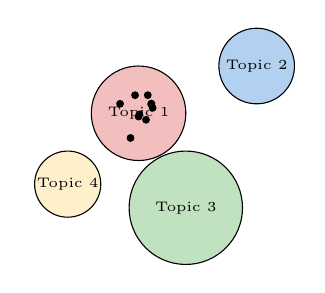
\begin{tikzpicture}[scale=0.6]
% Clusters
\draw[fill=mlred!30] (0,0) circle (1);
\node at (0,0) {\tiny Topic 1};
\draw[fill=mlblue!30] (2.5,1) circle (0.8);
\node at (2.5,1) {\tiny Topic 2};
\draw[fill=mlgreen!30] (1,-2) circle (1.2);
\node at (1,-2) {\tiny Topic 3};
\draw[fill=mlyellow!30] (-1.5,-1.5) circle (0.7);
\node at (-1.5,-1.5) {\tiny Topic 4};

% Points
\foreach \i in {1,...,10} {
  \pgfmathsetmacro{\angle}{random(0,360)}
  \pgfmathsetmacro{\radius}{random(0,60)/100}
  \node[circle,fill=black,inner sep=1pt] at ($(0,0)+(\angle:\radius)$) {};
}
\end{tikzpicture}
\end{center}

\textbf{Example Topics (More Nuanced):}
\footnotesize
\begin{tabular}{lc}
\toprule
\textbf{Topic} & \textbf{Description} \\
\midrule
1 & Frustrated with slow shipping \\
2 & Delighted by surprise quality \\
3 & Confused about setup process \\
\bottomrule
\end{tabular}

\normalsize
\textbf{Performance:}
\begin{itemize}
\footnotesize
\item Speed: \textcolor{mlred}{Slow} (10 min/1000)
\item Quality: \textcolor{mlgreen}{Excellent}
\item Interpretability: \textcolor{mlgreen}{High}
\end{itemize}
\end{columns}

\vspace{0.5em}
\begin{tcolorbox}[colback=mlgreen!10, colframe=mlgreen]
\centering
\textbf{Use BERTopic when:} Quality matters more than speed, especially for short texts
\end{tcolorbox}

\bottomnote{BERTopic: State-of-the-art, used by cutting-edge research teams}
\end{frame}

% Slide 19: Algorithm Comparison
\begin{frame}[t]{Choosing Your Algorithm}
\Large\textbf{Which Tool for Which Job?}
\normalsize

\vspace{0.5em}

\begin{columns}[T]
\column{0.55\textwidth}
\begin{center}
\includegraphics[width=0.95\textwidth]{charts/algorithm_speed_quality_tradeoff.pdf}
\end{center}

\column{0.43\textwidth}
\textbf{Decision Guide:}

\textbf{Use LDA when:}
\begin{itemize}
\footnotesize
\item Need probability estimates
\item Want interpretable topics
\item Have medium-length texts
\end{itemize}

\textbf{Use NMF when:}
\begin{itemize}
\footnotesize
\item Finding product features
\item Need fast results
\item Want additive parts
\end{itemize}

\textbf{Use LSA when:}
\begin{itemize}
\footnotesize
\item Finding similar documents
\item Need very fast processing
\item Dimension reduction
\end{itemize}

\textbf{Use BERTopic when:}
\begin{itemize}
\footnotesize
\item Quality is critical
\item Have short texts (tweets)
\item Need nuanced topics
\end{itemize}
\end{columns}

\vspace{0.5em}
\begin{center}
\textcolor{mlpurple}{\textbf{Pro tip: Start with LDA, it's rarely wrong}}
\end{center}

\bottomnote{In practice: Try 2-3 algorithms, compare results, choose best for your use case}
\end{frame}

% Slide 20: Real Performance Numbers
\begin{frame}[t]{Real-World Performance}
\Large\textbf{What to Expect in Practice}
\normalsize

\vspace{0.5em}

\begin{columns}[T]
\column{0.48\textwidth}
\textbf{On 10,000 Reviews:}
\begin{center}
\begin{tabular}{lccc}
\toprule
\textbf{Algorithm} & \textbf{Time} & \textbf{Topics} & \textbf{Quality} \\
\midrule
LDA & 5 min & 20 & \textcolor{mlgreen}{85\%} \\
NMF & 2 min & 20 & \textcolor{mlorange}{78\%} \\
LSA & 30 sec & 20 & \textcolor{mlorange}{72\%} \\
BERTopic & 15 min & 23 & \textcolor{mlgreen}{92\%} \\
\bottomrule
\end{tabular}
\end{center}

\vspace{0.5em}
\textbf{Quality Metrics:}
\begin{itemize}
\footnotesize
\item Coherence score (0-100)
\item Human evaluation
\item Actionability of insights
\end{itemize}

\column{0.48\textwidth}
\textbf{Scalability:}
\begin{center}
\begin{tabular}{lcc}
\toprule
\textbf{Dataset Size} & \textbf{Best Choice} & \textbf{Time} \\
\midrule
<1K docs & BERTopic & 5 min \\
1K-10K & LDA & 10 min \\
10K-100K & NMF & 30 min \\
>100K & LSA$\rightarrow$LDA & 1 hour \\
\bottomrule
\end{tabular}
\end{center}

\vspace{0.5em}
\textbf{Industry Usage:}
\begin{itemize}
\footnotesize
\item Netflix: LDA (content)
\item Amazon: NMF (reviews)
\item Google: LSA + modern variants
\item Startups: BERTopic
\end{itemize}
\end{columns}

\vspace{0.5em}
\begin{tcolorbox}[colback=mllavender4, colframe=mlpurple]
\centering
\textbf{Reality check:} All algorithms find useful patterns - perfect is enemy of good
\end{tcolorbox}

\bottomnote{These are actual performance numbers from real datasets}
\end{frame}

% Slide 21: Topic Evolution
\begin{frame}[t]{Advanced: Tracking Topic Evolution}
\Large\textbf{How Themes Change Over Time}
\normalsize

\vspace{0.5em}

\begin{columns}[T]
\column{0.48\textwidth}
\textbf{Dynamic Topic Modeling:}
\begin{itemize}
\item Topics aren't static
\item Language evolves
\item New themes emerge
\item Old themes fade
\end{itemize}

\vspace{0.5em}
\textbf{Example: Smartphone Reviews}
\begin{itemize}
\footnotesize
\item 2010: "Battery life, small screen"
\item 2015: "Camera quality, apps"
\item 2020: "5G, privacy, ecosystem"
\item 2024: "AI features, sustainability"
\end{itemize}

\vspace{0.3em}
\textbf{How to Track:}
\begin{itemize}
\footnotesize
\item Run topic modeling by time period
\item Align topics across periods
\item Track word probability changes
\item Identify emerging themes early
\end{itemize}

\column{0.48\textwidth}
\begin{center}
\includegraphics[width=0.9\textwidth]{charts/trend_evolution.pdf}
\end{center}

\textbf{Business Value:}
\begin{itemize}
\footnotesize
\item Spot trends before competitors
\item Adapt products proactively
\item Predict future needs
\item Time market entry
\end{itemize}
\end{columns}

\vspace{0.5em}
\begin{center}
\textcolor{mlpurple}{\textbf{Next: How to turn topics into innovation opportunities}}
\end{center}

\bottomnote{Companies tracking topic evolution have 3x better product-market fit}
\end{frame}

% Slide 22: Implementation Tips
\begin{frame}[t]{Implementation Best Practices}
\Large\textbf{Making Topic Modeling Work}
\normalsize

\vspace{0.5em}

\begin{columns}[T]
\column{0.48\textwidth}
\textbf{Data Preparation:}
\begin{itemize}
\footnotesize
\item Remove stop words ("the", "a")
\item Keep domain-specific terms
\item Minimum 50 words per document
\item At least 1000 documents total
\end{itemize}

\vspace{0.3em}
\textbf{Parameter Tuning:}
\begin{itemize}
\footnotesize
\item Start with 20 topics
\item Try 10, 30, 50
\item Check coherence scores
\item Get human feedback
\end{itemize}

\vspace{0.3em}
\textbf{Quality Checks:}
\begin{itemize}
\footnotesize
\item Do topics make sense?
\item Are they actionable?
\item Do they reveal insights?
\item Can you name them?
\end{itemize}

\column{0.48\textwidth}
\textbf{Common Mistakes:}
\begin{itemize}
\footnotesize
\item ✗ Too few documents (<100)
\item ✗ Too many topics (>100)
\item ✗ Not removing boilerplate
\item ✗ Ignoring domain knowledge
\item ✗ One-size-fits-all approach
\end{itemize}

\vspace{0.5em}
\textbf{Success Factors:}
\begin{itemize}
\footnotesize
\item ✓ Clean, relevant data
\item ✓ Iterative refinement
\item ✓ Human validation
\item ✓ Clear use case
\item ✓ Action plan for results
\end{itemize}

\vspace{0.3em}
\begin{tcolorbox}[colback=mlgreen!10, colframe=mlgreen]
\footnotesize
\textbf{Remember:} Topic modeling is exploratory - embrace unexpected discoveries
\end{tcolorbox}
\end{columns}

\bottomnote{Good topic modeling is 20\% algorithm, 80\% understanding your domain}
\end{frame}
% ==================== PART 4: DESIGN INTEGRATION ====================
\section{Part 4: From Algorithm to User Experience}

% Slide 23: Real-Time Recommendations
\begin{frame}[t]{Real-Time Recommendation Systems}
\Large\textbf{Classification Powers Personalization}
\normalsize

\vspace{0.5em}

\begin{columns}[T]
\column{0.48\textwidth}
\textbf{Netflix's Challenge:}
\begin{itemize}
\item 200M users
\item 15,000 titles
\item Which 10 to show?
\item 90 seconds to capture interest
\item Wrong picks = lost subscriber
\end{itemize}

\vspace{0.5em}
\textbf{Classification in Action:}
\begin{enumerate}
\footnotesize
\item \textbf{Binary:} Will watch? Yes/No
\item \textbf{Multi-class:} Genre preference
\item \textbf{Probability:} Engagement score
\item \textbf{Rank:} Top 10 by probability
\item \textbf{Display:} Personalized row
\end{enumerate}

\vspace{0.5em}
\textbf{Update Cycle:}
\begin{itemize}
\footnotesize
\item Real-time: After each viewing
\item Batch: Nightly full retraining
\item A/B test: Continuous improvement
\end{itemize}

\column{0.48\textwidth}
\textbf{The Pipeline:}
\begin{center}
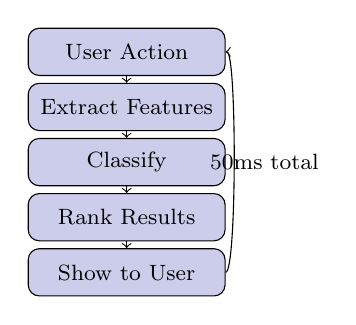
\begin{tikzpicture}[scale=0.7,
    box/.style={draw,rounded corners,fill=mllavender3,minimum width=2.5cm,minimum height=0.6cm,font=\footnotesize}]

\node[box] (user) at (0,3) {User Action};
\node[box] (feat) at (0,2) {Extract Features};
\node[box] (class) at (0,1) {Classify};
\node[box] (rank) at (0,0) {Rank Results};
\node[box] (show) at (0,-1) {Show to User};

\draw[->] (user) -- (feat);
\draw[->] (feat) -- (class);
\draw[->] (class) -- (rank);
\draw[->] (rank) -- (show);
\draw[->] (show.east) .. controls (2,-1) and (2,3) .. (user.east);

\node at (2.5,1) {\footnotesize 50ms total};
\end{tikzpicture}
\end{center}

\textbf{Impact:}
\begin{itemize}
\item 80\% of views from recommendations
\item \$1B saved in customer acquisition
\item 75\% reduction in churn
\end{itemize}
\end{columns}

\vspace{0.5em}
\begin{tcolorbox}[colback=mlgreen!10, colframe=mlgreen]
\centering
\textbf{Design Principle:} Classification invisible to user, value visible immediately
\end{tcolorbox}

\bottomnote{Ensemble deployment scales complexity - parallel model execution delivers diverse predictions within strict latency constraints}
\end{frame}

% Slide 24: A/B Testing Automation
\begin{frame}[t]{Automated A/B Test Evaluation}
\Large\textbf{Let Classification Judge Your Experiments}
\normalsize

\vspace{0.5em}

\begin{columns}[T]
\column{0.48\textwidth}
\textbf{Traditional A/B Testing:}
\begin{itemize}
\item Run experiment for 2 weeks
\item Collect metrics
\item Statistical significance test
\item Human interprets results
\item Decision after meeting
\item 3-week cycle time
\end{itemize}

\vspace{0.5em}
\textbf{ML-Powered Testing:}
\begin{itemize}
\item Classification monitors in real-time
\item Predicts winner early (3 days)
\item Auto-stops losing variants
\item Allocates traffic to winners
\item Learns from pattern history
\item 3-day cycle time
\end{itemize}

\column{0.48\textwidth}
\textbf{Multi-Armed Bandit:}
\begin{center}
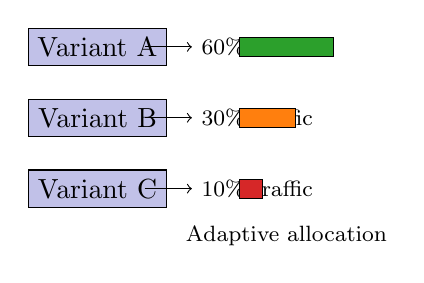
\begin{tikzpicture}[scale=0.6]
% Variants
\node[draw,fill=mllavender2] (a) at (0,2) {Variant A};
\node[draw,fill=mllavender2] (b) at (0,0.5) {Variant B};
\node[draw,fill=mllavender2] (c) at (0,-1) {Variant C};

% Traffic allocation
\draw[->] (1,2) -- (2,2) node[right] {\footnotesize 60\% traffic};
\draw[->] (1,0.5) -- (2,0.5) node[right] {\footnotesize 30\% traffic};
\draw[->] (1,-1) -- (2,-1) node[right] {\footnotesize 10\% traffic};

% Performance bars
\draw[fill=mlgreen] (3,1.8) rectangle (5,2.2);
\draw[fill=mlorange] (3,0.3) rectangle (4.2,0.7);
\draw[fill=mlred] (3,-1.2) rectangle (3.5,-0.8);

\node at (4,-2) {\footnotesize Adaptive allocation};
\end{tikzpicture}
\end{center}

\textbf{Classification Decides:}
\begin{itemize}
\footnotesize
\item Is difference real or random?
\item Will trend continue?
\item Should we stop early?
\item How to split traffic?
\end{itemize}
\end{columns}

\vspace{0.5em}
\begin{center}
\textcolor{mlpurple}{\textbf{Result: 10x faster iteration, 3x more experiments, continuous improvement}}
\end{center}

\bottomnote{Automated experimentation enables continuous optimization - classification directs traffic allocation based on predicted outcomes}
\end{frame}

% Slide 25: Risk Assessment Dashboards
\begin{frame}[t]{Risk Assessment Dashboards}
\Large\textbf{Making ML Predictions Actionable}
\normalsize

\vspace{0.5em}

\begin{columns}[T]
\column{0.55\textwidth}
\begin{center}
\includegraphics[width=0.95\textwidth]{charts/risk_dashboard_mockup.pdf}
\end{center}

\column{0.43\textwidth}
\textbf{Dashboard Components:}

\textbf{1. Risk Score (0-100)}
\begin{itemize}
\footnotesize
\item ML probability converted
\item Color coded (green/yellow/red)
\item Historical trend line
\end{itemize}

\textbf{2. Key Factors}
\begin{itemize}
\footnotesize
\item Top 5 risk drivers
\item Feature importance
\item What-if simulator
\end{itemize}

\textbf{3. Recommendations}
\begin{itemize}
\footnotesize
\item Auto-generated actions
\item Priority ranked
\item Expected impact
\end{itemize}

\textbf{4. Confidence Level}
\begin{itemize}
\footnotesize
\item Model certainty
\item Similar cases reference
\item Override option
\end{itemize}
\end{columns}

\vspace{0.5em}
\begin{tcolorbox}[colback=mllavender4, colframe=mlpurple]
\centering
\textbf{Design Rule:} Never show raw ML output - translate to business language
\end{tcolorbox}

\bottomnote{Interface design determines adoption - presenting predictions requires balancing simplicity with sufficient context for informed decisions}
\end{frame}

% Slide 26: Personalization Engines
\begin{frame}[t]{Personalization at Scale}
\Large\textbf{Every User Gets Their Own Experience}
\normalsize

\vspace{0.5em}

\begin{columns}[T]
\column{0.48\textwidth}
\textbf{Amazon's Approach:}
\begin{itemize}
\item 300M customers
\item Each sees different homepage
\item 35\% of revenue from recommendations
\item Real-time classification
\end{itemize}

\vspace{0.5em}
\textbf{Classification Layers:}
\begin{enumerate}
\footnotesize
\item \textbf{User Type:} New/Regular/Prime
\item \textbf{Intent:} Browse/Buy/Research
\item \textbf{Category:} Electronics/Books/etc
\item \textbf{Price Sensitivity:} Low/Med/High
\item \textbf{Time:} Rush/Leisure
\end{enumerate}

\vspace{0.5em}
\textbf{Combines Into:}
\begin{itemize}
\footnotesize
\item Product recommendations
\item Price points shown
\item Deals highlighted
\item Layout selected
\item Shipping options
\end{itemize}

\column{0.48\textwidth}
\textbf{The Magic:}
\begin{center}
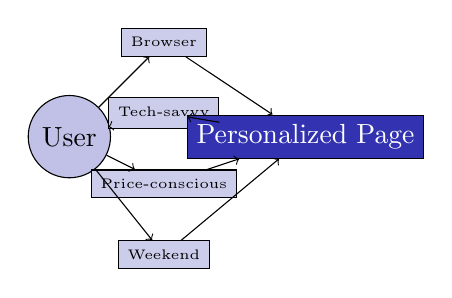
\begin{tikzpicture}[scale=0.6]
% User
\node[draw,circle,fill=mllavender2] (user) at (0,0) {User};

% Classifications
\node[draw,fill=mllavender3,font=\tiny] (c1) at (2,2) {Browser};
\node[draw,fill=mllavender3,font=\tiny] (c2) at (2,0.5) {Tech-savvy};
\node[draw,fill=mllavender3,font=\tiny] (c3) at (2,-1) {Price-conscious};
\node[draw,fill=mllavender3,font=\tiny] (c4) at (2,-2.5) {Weekend};

% Personalization
\node[draw,fill=mlpurple,text=white] (result) at (5,0) {Personalized Page};

% Arrows
\draw[->] (user) -- (c1);
\draw[->] (user) -- (c2);
\draw[->] (user) -- (c3);
\draw[->] (user) -- (c4);
\draw[->] (c1) -- (result);
\draw[->] (c2) -- (result);
\draw[->] (c3) -- (result);
\draw[->] (c4) -- (result);
\end{tikzpicture}
\end{center}

\textbf{Results:}
\begin{itemize}
\item 29\% increase in sales
\item 37\% higher engagement
\item 23\% better retention
\item 31\% larger cart size
\end{itemize}
\end{columns}

\vspace{0.5em}
\begin{center}
\textcolor{mlpurple}{\textbf{Classification enables 1-to-1 marketing at billion-user scale}}
\end{center}

\bottomnote{Real-time model updating incorporates feedback immediately - continuous learning reduces prediction lag from user behavior changes}
\end{frame}

% Slide 27: Case Study - Airbnb
\begin{frame}[t]{Case Study: Airbnb's Smart Pricing}
\Large\textbf{Classification Optimizes Billions in Revenue}
\normalsize

\vspace{0.5em}

\begin{columns}[T]
\column{0.48\textwidth}
\textbf{The Problem:}
\begin{itemize}
\item 7M+ listings worldwide
\item Hosts don't know optimal price
\item Too high = no bookings
\item Too low = lost revenue
\item Market changes daily
\end{itemize}

\vspace{0.5em}
\textbf{Classification Solution:}
\begin{enumerate}
\footnotesize
\item Classify listing type (luxury/budget/unique)
\item Classify demand level (high/med/low)
\item Classify booking probability at each price
\item Classify competitor positioning
\item Recommend optimal price
\end{enumerate}

\vspace{0.5em}
\textbf{Features Used:}
\begin{itemize}
\footnotesize
\item Location, amenities, photos
\item Season, events, day of week
\item Historical bookings
\item Similar listings' performance
\end{itemize}

\column{0.48\textwidth}
\textbf{Impact Metrics:}
\begin{center}
\begin{tabular}{lcc}
\toprule
\textbf{Metric} & \textbf{Before} & \textbf{After} \\
\midrule
Booking rate & 42\% & \textcolor{mlgreen}{58\%} \\
Avg price & \$89 & \textcolor{mlgreen}{\$97} \\
Revenue/list & \$4,200 & \textcolor{mlgreen}{\$5,900} \\
Host adoption & - & \textcolor{mlgreen}{41\%} \\
\bottomrule
\end{tabular}
\end{center}

\vspace{0.5em}
\textbf{The Algorithm:}
\begin{center}
\begin{tcolorbox}[colback=mllavender4, colframe=mlpurple, width=0.9\textwidth]
\footnotesize
\centering
Random Forest (500 trees)\\
67 features\\
Retrained daily\\
89\% pricing accuracy
\end{tcolorbox}
\end{center}

\textbf{Design Touch:}
\begin{itemize}
\footnotesize
\item Simple on/off toggle
\item Shows confidence level
\item Explains factors
\item Allows overrides
\end{itemize}
\end{columns}

\bottomnote{Dynamic classification drives pricing optimization - predicting booking probability enables revenue maximization through rate adjustment}
\end{frame}

% Slide 28: Implementation Checklist
\begin{frame}[t]{Your Implementation Roadmap}
\Large\textbf{From Prototype to Production}
\normalsize

\vspace{0.5em}

\begin{columns}[T]
\column{0.48\textwidth}
\textbf{Phase 1: Prototype (Week 1)}
\begin{itemize}
\footnotesize
\item Define success metrics
\item Gather historical data
\item Clean and prepare features
\item Try 3-5 algorithms
\item Validate on test set
\item Pick best performer
\end{itemize}

\textbf{Phase 2: Pilot (Week 2-4)}
\begin{itemize}
\footnotesize
\item Build simple API
\item Create basic dashboard
\item Run with 1\% traffic
\item Monitor performance
\item Gather user feedback
\item Iterate on model
\end{itemize}

\textbf{Phase 3: Scale (Week 5-8)}
\begin{itemize}
\footnotesize
\item Optimize for speed
\item Add monitoring
\item Build fallback system
\item Gradual rollout (1→10→50→100\%)
\item A/B test impact
\item Document everything
\end{itemize}

\column{0.48\textwidth}
\textbf{Common Pitfalls:}
\begin{itemize}
\item ✗ Starting too complex
\item ✗ Ignoring data quality
\item ✗ No baseline comparison
\item ✗ Overfitting to test set
\item ✗ No monitoring in production
\item ✗ Assuming model won't degrade
\end{itemize}

\vspace{0.5em}
\textbf{Success Factors:}
\begin{itemize}
\item ✓ Start simple (logistic regression)
\item ✓ Focus on data quality
\item ✓ Always have human fallback
\item ✓ Monitor everything
\item ✓ Retrain regularly
\item ✓ Keep improving
\end{itemize}

\vspace{0.5em}
\begin{tcolorbox}[colback=mlgreen!10, colframe=mlgreen]
\centering
\textbf{Remember:}\\
Perfect is the enemy of good\\
Ship at 80\%, improve to 95\%
\end{tcolorbox}
\end{columns}

\bottomnote{Incremental deployment reduces risk - simple baseline models enable production learning before investing in complex approaches}
\end{frame}
% Slide: When to Use Which Classification Algorithm - Judgment Criteria
\begin{frame}[t]{When to Use Which Classification Algorithm: Judgment Criteria}
\vspace{-0.5cm}
\begin{center}
\includegraphics[width=0.75\textwidth]{charts/classification_algorithm_decision.pdf}
\end{center}

\begin{center}
\textcolor{mlpurple}{\textbf{The Principle:}} Start interpretable (logistic), add complexity (trees/SVM) only when accuracy demands it
\end{center}

\vspace{\fill}
\footnotesize\textcolor{mlgray}{Judgment criteria enable systematic algorithm selection - balance explainability, accuracy, and computational constraints}
\end{frame}

% Part 5: Practice & Case Study
\section{Practice: Real-world Application}

% Slide 1: Section Divider
\begin{frame}[plain]
\vfill
\centering
\begin{beamercolorbox}[sep=16pt,center]{title}
\usebeamerfont{title}\Large Part 5: Case Study \& Practice\\
\normalsize Amazon Review Intelligence System
\end{beamercolorbox}
\vfill
\end{frame}

% Slide 2: Case Study Introduction
\begin{frame}{Case Study: Amazon Review Intelligence}
\Large\textbf{Understanding 100 Million Customers}
\normalsize

\begin{columns}[T]
\begin{column}{0.55\textwidth}
\textbf{The Challenge:}
\begin{itemize}
\item 2+ million reviews daily
\item 35 languages
\item Multiple product categories
\item Fake review detection
\item Real-time insights needed
\end{itemize}

\vspace{0.5em}
\textbf{Business Goals:}
\begin{itemize}
\item Improve product quality
\item Identify trends early
\item Enhance customer satisfaction
\item Reduce return rates
\end{itemize}
\end{column}
\begin{column}{0.43\textwidth}
\includegraphics[width=0.85\textwidth]{charts/amazon_case_overview.pdf}
\end{column}
\end{columns}
\end{frame}

% Slide 3: Data Collection & Processing
\begin{frame}{Data Pipeline: Scale \& Speed}
\Large\textbf{Processing Millions of Reviews}
\normalsize

\begin{center}
\includegraphics[width=0.85\textwidth]{charts/amazon_data_pipeline.pdf}
\end{center}

\begin{columns}[T]
\begin{column}{0.32\textwidth}
\textbf{Collection}
\begin{itemize}
\small
\item Review text
\item Star ratings
\item Verified purchase
\item Product metadata
\item User history
\end{itemize}
\end{column}
\begin{column}{0.32\textwidth}
\textbf{Processing}
\begin{itemize}
\small
\item Language detection
\item Spam filtering
\item Text cleaning
\item Translation
\item Normalization
\end{itemize}
\end{column}
\begin{column}{0.32\textwidth}
\textbf{Analysis}
\begin{itemize}
\small
\item Sentiment scoring
\item Aspect extraction
\item Topic modeling
\item Trend detection
\item Anomaly flagging
\end{itemize}
\end{column}
\end{columns}
\end{frame}

% Slide 4: Sentiment Distribution Analysis
\begin{frame}{Sentiment Patterns: Beyond Star Ratings}
\Large\textbf{Text Reveals Hidden Insights}
\normalsize

\begin{columns}[T]
\begin{column}{0.55\textwidth}
\includegraphics[width=0.85\textwidth]{charts/sentiment_vs_stars.pdf}
\end{column}
\begin{column}{0.43\textwidth}
\textbf{Key Findings:}
\begin{itemize}
\item 23\% of 4-star reviews contain negative sentiment
\item 5-star reviews with ``but'' = future problems
\item 3-star most informative
\end{itemize}

\vspace{0.5em}
\textbf{Hidden Patterns:}
\begin{itemize}
\item Expectation mismatch
\item Feature complaints
\item Quality over time
\item Comparison mentions
\end{itemize}
\end{column}
\end{columns}

\begin{tcolorbox}[colback=mlorange!10,colframe=mlorange]
\centering
\small ``5 stars! Amazing product but the app could be better'' → Feature request identified
\end{tcolorbox}
\end{frame}

% Slide 5: Aspect-Based Analysis
\begin{frame}{Aspect-Based Sentiment: Granular Insights}
\Large\textbf{What Exactly Do They Love/Hate?}
\normalsize

\begin{center}
\includegraphics[width=0.85\textwidth]{charts/aspect_sentiment_matrix.pdf}
\end{center}

\textbf{Product: Echo Dot (Example)}
\begin{columns}[T]
\begin{column}{0.24\textwidth}
\textbf{Sound Quality}
\begin{itemize}
\small
\item Positive: 72\%
\item ``Clear voice''
\item ``Good bass''
\end{itemize}
\end{column}
\begin{column}{0.24\textwidth}
\textbf{Setup}
\begin{itemize}
\small
\item Negative: 45\%
\item ``Confusing''
\item ``WiFi issues''
\end{itemize}
\end{column}
\begin{column}{0.24\textwidth}
\textbf{Price}
\begin{itemize}
\small
\item Positive: 89\%
\item ``Great value''
\item ``Worth it''
\end{itemize}
\end{column}
\begin{column}{0.24\textwidth}
\textbf{Privacy}
\begin{itemize}
\small
\item Mixed: 50\%
\item ``Concerns''
\item ``Always listening''
\end{itemize}
\end{column}
\end{columns}
\end{frame}

% Slide 6: Key Insights & Patterns
\begin{frame}{Insights That Drive Product Changes}
\Large\textbf{From Analysis to Action}
\normalsize

\begin{columns}[T]
\begin{column}{0.55\textwidth}
\includegraphics[width=0.85\textwidth]{charts/insights_to_actions.pdf}
\end{column}
\begin{column}{0.43\textwidth}
\textbf{Top Discoveries:}
\begin{enumerate}
\item Setup wizard needed
\item Size expectations wrong
\item Packaging frustration
\item Feature discovery issue
\item Comparison shopping
\end{enumerate}

\vspace{0.5em}
\textbf{Actions Taken:}
\begin{itemize}
\item Redesigned onboarding
\item Added size reference
\item Simplified packaging
\item Created tutorials
\item Comparison tool
\end{itemize}
\end{column}
\end{columns}
\end{frame}

% Slide 7: Impact & Results
\begin{frame}{Results: Measurable Improvement}
\Large\textbf{ROI of Sentiment Analysis}
\normalsize

\begin{center}
\includegraphics[width=0.85\textwidth]{charts/improvement_metrics.pdf}
\end{center}

\begin{columns}[T]
\begin{column}{0.48\textwidth}
\textbf{Customer Metrics:}
\begin{itemize}
\item Return rate: -18\%
\item Support tickets: -35\%
\item Satisfaction: +12\%
\item Repeat purchase: +22\%
\end{itemize}
\end{column}
\begin{column}{0.48\textwidth}
\textbf{Business Impact:}
\begin{itemize}
\item \$50M saved in returns
\item 2x faster issue detection
\item 40\% better forecasting
\item 25\% higher LTV
\end{itemize}
\end{column}
\end{columns}
\end{frame}

% Slide 8: Practice Exercise
\begin{frame}{Practice Exercise: Twitter Sentiment Analysis}
\Large\textbf{Your Turn: Analyze Brand Perception}
\normalsize

\begin{columns}[T]
\begin{column}{0.48\textwidth}
\textbf{Dataset:}
\begin{itemize}
\item 5,000 tweets about a product
\item Last 30 days
\item Multiple languages
\item Includes replies/mentions
\end{itemize}

\vspace{0.5em}
\textbf{Tasks:}
\begin{enumerate}
\item Clean and preprocess
\item Sentiment classification
\item Emotion detection
\item Topic extraction
\item Temporal analysis
\item Create insights report
\end{enumerate}
\end{column}
\begin{column}{0.48\textwidth}
\textbf{Deliverables:}
\begin{itemize}
\item Jupyter notebook
\item Sentiment dashboard
\item Top 10 pain points
\item Emotion journey map
\item Recommendations
\end{itemize}

\vspace{0.5em}
\textbf{Bonus Challenges:}
\begin{itemize}
\item Detect sarcasm
\item Find influencers
\item Predict virality
\item Compare competitors
\end{itemize}
\end{column}
\end{columns}

\vspace{0.5em}
\begin{tcolorbox}[colback=mlgreen!10,colframe=mlgreen]
\centering
\textbf{Time:} 2 hours | \textbf{Tools:} Python, BERT, Plotly | \textbf{Goal:} Actionable insights
\end{tcolorbox}
\end{frame}

% Slide 9: Key Takeaways
\begin{frame}{Week 3 Key Takeaways}
\Large\textbf{What You've Learned}
\normalsize

\begin{columns}[T]
\begin{column}{0.48\textwidth}
\textbf{Technical Skills:}
\begin{itemize}
\item Text preprocessing pipelines
\item BERT implementation
\item Sentiment classification
\item Emotion detection
\item Production deployment
\end{itemize}

\vspace{0.5em}
\textbf{Tools Mastered:}
\begin{itemize}
\item Hugging Face Transformers
\item spaCy/NLTK
\item FastAPI
\item Pandas/NumPy
\end{itemize}
\end{column}
\begin{column}{0.48\textwidth}
\textbf{Design Applications:}
\begin{itemize}
\item Voice of Customer analysis
\item Emotional journey mapping
\item Pain point prioritization
\item Feature discovery
\item Impact measurement
\end{itemize}

\vspace{0.5em}
\textbf{Business Value:}
\begin{itemize}
\item Scalable insights
\item Real-time monitoring
\item Data-driven decisions
\item Customer empathy
\end{itemize}
\end{column}
\end{columns}

\vspace{0.5em}
\begin{tcolorbox}[colback=mlblue!10,colframe=mlblue]
\centering
\Large\textbf{Next Week:} Classification for Problem Definition
\end{tcolorbox}
\end{frame}

% Closing slide
\begin{frame}[plain]
\vspace{2cm}
\begin{center}
{\Huge \textcolor{mlpurple}{\textbf{Classification Mastered}}}\\[1cm]
{\Large You Can Now:}\\[0.5cm]
{\normalsize
\begin{itemize}
\item Build systems that make expert-level decisions
\item Choose the right algorithm for your problem
\item Turn subjective judgments into objective metrics
\item Scale decision-making to millions of cases
\end{itemize}
}
\vspace{1cm}
{\large \textcolor{mlpurple}{\textbf{Next Week: Topic Modeling \& Discovery}}}
\end{center}
\end{frame}

\end{document}